\chapter{Исследование и построение решения задачи}
\label{sec:Chapter3} \index{Chapter3}


\section{Показатели качества РЛИ}

	Важным показателем качества синтеза РЛИ является пространственное разрешение, которое характеризует наименьшее расстояние для раздельного воспроизведения изображения двух точечных объектов. При разнесении точек в пространстве посередине между ними в изображении возникает локальный минимум интенсивности (провал). Разрешение определяется величиной наименьшего расстояния, на котором достоверно обнаруживается этот провал [Занин]:
	
\begin{equation}
    \Delta y = k_p*R_g,
\end{equation}

где $ \Delta y $ - расстояние между точечными объектами (линейное разрешение), $ k_p $ - коэффициент ухудшения разрешения относительно идеального, $ R_g $ - предельная разрешающая способность РСА. 
	Данное расстояние зависит от контраста наблюдаемого объекта, отношения сигнал-шум и ошибок информационного тракта. Целью синтеза РЛИ является сделать пространственное разрешение равным предельной разрешающей способности РСА.
	
	Общепринятым подходом для оценки разрешения РЛИ является измерение ширины профиля квадрата функции рассеяния точки (ФРТ) по уровню -3 дБ в направлениях азимута и дальности. Также существуют и другие методы, такие как измерение пространственного разрешения по автокорреляционной функции  изображения [2], оценка разрешения по протяженным линейным объектам [2], использование элементов алгоритма PGA [2]. Также в [] предложено измерять разрешение по формуле:
	
\begin{equation}
    \Delta y = k_p*R_g,
\end{equation}
	
	Помимо этого в [] предложено измерять разрешение по периодическим структурам.	
	
	Преимуществом анализа ФРТ является то, что помимо разрешения, с помощью него можно вычислить и другие параметры РЛИ, такие как контраст, отношение сигнал/шум и др. Так как радиолокационые системы (РЛС) являются линейными [1 с.59 Wong], то есть вид их передаточных функций не зависит от величины входного воздействия, то естественно исследовать ФРТ как отклик от единичного импульса, который формируется тест объектом. В РСА таким тест объектом является одиночный, изолированный рассеиватель, такой как уголковый отражатель. Особенность его заключается в том, что падающий на него зондирующий импульс отражается точно в противоположном направлении. Такой малый, дискретный рассеиватель ещё называют точечной целью. Большинство параметров РЛС измеряются по отклику от такой цели. Откликом точечной цели является sinc-like функция [1].

	Идея данной работы заключается в использовании в качестве тест объектов псевдоточечные цели, то есть цели, для которых заведомо неизвестно, являются ли они одиночными, изолированными, то есть точечными. При большой выборке данных целей (100 - 1000 штук), в ней могут оказаться как точечные, так и неточечные. Соответсвенно профиль функции рассеяния псевдоточечной цели будет шире чем профиль ФРТ, так как функция рассеяния псевдоточечной цели будет суммой ФРТ, сдвинутых друг относительно друга на $ {\delta x < \Delta y} $. 

	Далее рассмотрим механизм формирования отклика от псевдоточечной цели. Логично, предположить, что данный отклик будет суммой откликов от точечных целей, раз мы считаем точечную цель неделимой, единичной структурой.
	
\section{Модель формирования псевдоточечных целей}

	Точечные цели образуют псевдоточечные цели, если они расположены на расстоянии меньше разрешающей способности радиолокатора. Возьмём точечные цели с разрешением 0.8838 м и расположим случайным образом на фиксированной сцене. Геометрия получившейся модели показана на рисунке \ref{fig:pseudo_targets}.
	
	
\begin{figure}[ht]
    \centering
    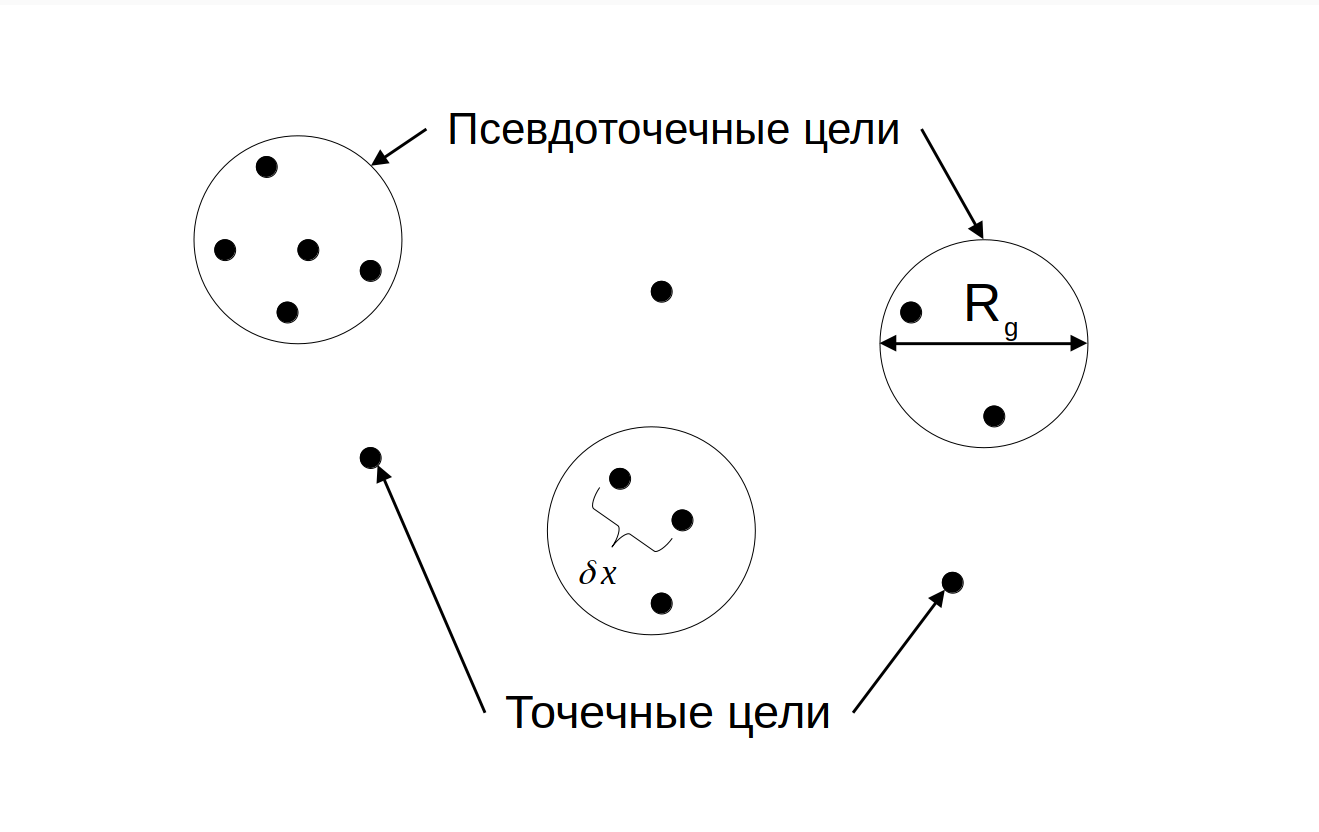
\includegraphics[width=0.8\textwidth]{pseudo_targets.png}
    \caption{Модель формировния псевдоточечных целей}
    \label{fig:pseudo_targets}
\end{figure}


	Те точечные цели, что попали в круг радиуса  $R_g$  (разрешающей способности радиолокатора) , образует единый отклик псевдоточечной цели. Сгенерируем случайным образом отклонения $ \delta x $ и количество попавших в круг целей и рассчитаем разрешения получившихся псевдоточечных целей. После этого найдем максимум распределения. Код модели, реализованный на языке Python 3 представлен ниже.
	
\begin{verbatim}
	import matplotlib.pyplot as plt
	import numpy as np
	from scipy.signal import find_peaks
	from scipy.signal import peak_widths

	def point_target(x, a):
	    """
	    Вычисляет квадрат отклика точеченой цели
	    :param x: массив действительных чисел, числовая ось
	    :param a: параметр, отвечающий за разрешение
	    :return: массив отклика точечной цели
	    """
	    arg = np.pi*x/a
	    return pow(np.sin(arg)/arg, 2)

	def irw(signal):
	    """
	    Вычисляет IRW (impulse response width) входного сигнала
	    :param signal: массив действительных чисел, функция вида sin(x)/x
	    :return: значение IRW сигнала
	    """
	    # Находим локальные максимумы
	    peaks = find_peaks(signal)[0]
	    # Мерим их ширину на высоте 1/sqrt(2)
	    width = peak_widths(signal, peaks, rel_height=1 - pow(10, -0.3))[0]
	    # Отбираем максимальную ширину - ширину главного лепестка
	    irw = np.max(width)
	    return irw

	def max_distr(arr):
	    """
	    Вычисляет максимум распределения массива arr
	    :param arr: массив действительных чисел
	    :return: максимум распределения
	    """
	    arr.sort()    
	    while len(arr) > 1:    
		border = (arr[0] + arr[-1])/2       
		if all([x == border for x in arr]):
		    break            
		left = []
		right = []        
		for item in arr:
		    if item < border:
		        left.append(item)
		    else:
		        right.append(item)            
		if len(right) > len(left):
		    arr = right
		else:
		    arr = left		    
	    return arr[0]
		
	a = 1 
	start = -10
	stop = 10
	count = 1000
	scale = (stop - start)/count

	t = np.linspace(start, stop, count)

	dx = np.random.rand(1000)
	dx = (2*dx - 1)*a
	res = []

	for n in np.random.randint(1, 10, 1000):
	    s = [0]*len(t)
	    for delta in np.random.choice(dx, n):
		s += point_target(t + delta, a)        
	    res.append(scale*irw(s))

	print("Разрешение точечной цели:",  round(scale*irw(point_target(t, a)), 4))
	print("Максимум распределения разрешений псевдоточечных целей", round(max_distr(res), 4))
\end{verbatim}

	График получившегося распределния представлен нна рисунке \ref{fig:pseudo_distr}.

\begin{figure}[ht]
    \centering
    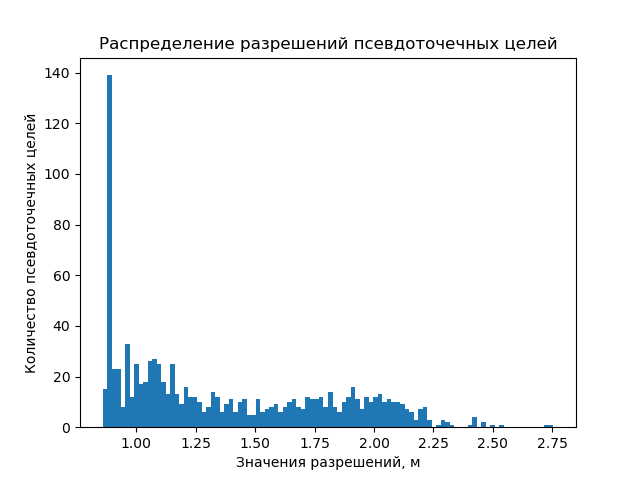
\includegraphics[width=0.8\textwidth]{pseudo_distr.png}
    \caption{Гистограмма распределния разрешений псевдоточечных целей}
    \label{fig:pseudo_distr}
\end{figure}

	Таким образом, максимум распределения разрешений псевдоточечных целей оказалось равно 0.8836, что отличается от эталонного не более чем на 0.03\%. Исходя из этого можно сделать вывод, что статистический анализ псевдоточечных целей даёт результаты очень близкие к реальным.

\section{Алгоритм поиска псевдоточечных целей на РЛИ}

	Алгоритм автоматического поиска псевдоточечных целей заключается в нахождении центров их откликов. В [Automatic point...] предложен алгоритм поиска, который заключается в вычислении свертки областей РЛИ с заранее сгенерированными квадратными матрицами, которые задают направления "лучей" отклика. У него есть ряд недостатков:
	
	1. Свертка применяется ко всем областям РЛИ
	
	2. Заранее сгенерированные матрицы имеют ограниченное количество направлений
	
	Данные проблемы решаются с помощью выделения наиболее информативных областей и использовании в качестве свёрточных матриц автокорреляционную функцию изображения.

\subsection{Выделение информативных участков изображения}

	Вычисление свёртки - ресурсозатратная операция для компьютера. Нецелесообразно производить вычисления на областях с высоким уровнем шума или на слабоотражающих участках, так как результат свёртки будет неопределен. Для первичной фильтрации входного изображения используются гистограммные признаки [prett]. В начале входное изображение разбивается на равные участки путем создания двумерной сетки. Далее для каждого участка вычисляется гистограммный признак и на основании его значения делается вывод. Всего было протестировано 6 признаков: среднее, дисперсия, коэффициент асимметрии, кожффициент эксцесса, энергия, энтропия. Однако наибольшей информативностью обладает коэффициент эксцесса. Данный вывод был сделан на основе решения задачи бинарной классификация, где правилом классификации выступало отклонение разрешения псевдоточечной цели от истинной. Таким образом, удалось выяснить, что на участках изображения со значением коэффициента эксцеса больше 10 имеют с большей вероятностью могут находится псевдоточечные цели с разрешением, близким к истинному. Результат бинарной классификации представлен на рисунке \ref{fig:binary_classification}, где зелеными звездочками помечены те учатки изображения, на которых имеются уголковые отражатели. 
	
\begin{figure}[ht]
    \centering
    
\includegraphics[width=0.8\textwidth]{binary_classification.png}
    \caption{Бинарная классификация}
    \label{fig:binary_classification}
\end{figure}

\subsection{Свёрточная матрица на основе автокорреляционной функции изображения}

	Вычисление автокорреляционной функции (АКФ) является ключевым элементом в обработке РЛИ: она используется для оценки разрешающей способности РСА, в методе автофокусировки, в оценке когерентности и шумов. По определению автокорреляционная функция комплексного изображения задается формулой:
	
\begin{equation}
    R_{II}(\Delta x, \Delta y) = \iint_{-\infty}^{\infty} I(x, y) \cdot I^*(x - \Delta x, y - \Delta y) \, dx \, dy
\end{equation}

где:
\begin{itemize}
	\item $I(x, y)$ - комплексное изображение,
	\item $I^*(x - \Delta x, y - \Delta y)$ - комплексно сопряженное изображение, сдвинутое на $(\Delta x, \Delta y)$,
	\item $\Delta x, \Delta y$ - пространственные сдвиги по осям $x$ и $y$ соответственно.
\end{itemize}

	На практике АКФ часто вычисляется через быстрое преобразование Фурье (БПФ) для ускорения расчётов:

	1. Вычисляется Фурье-образ изображения \(\mathcal{F}\{I\}\).
	2. Находится спектр мощности: \(S = |\mathcal{F}\{I\}|^2\).
	3. Обратное Фурье0преобразование от \(S\) даёт АКФ
	
	Или же сокращенно:
	
\begin{equation}
    \text{АКФ} = \mathrm{IFFT}(|\mathrm{FFT}(I)|^2)
\end{equation}	

	В радиолокации существует глубокая аналогия между АКФ и ФРТ. Обе функции описывают пространственное распределение энергии волнового фронта после взаимодействия с системой.
	
	ФРТ описывается функцией sinc:
	
\begin{equation}
    I(\theta) \sim \text{sinc}^2\left(\frac{\pi L \sin\theta}{\lambda}\right)
\end{equation}

	АКФ линейно-частотно модулированного (ЛЧМ) сигнала с полосой B:
	
\begin{equation}
    R{\tau} \sim \text{sinc}(\pi B \tau)
\end{equation}

	Пространственное разрешение обратно пропорциональна шиирине главного лепестка АКФ, что верно и для ФРТ. Таким образом, корреляция между ФРТ и АКФ будет иметь значение близкое к 1. Поэтому целесообразно использовать АКФ как свёрточную матрицу для нахождения псевдоточечных целей. Примеры АКФ и ФРТ предствалены на рисунках \ref{fig:acf} и ...:
	

\begin{figure}[ht]
    \centering
    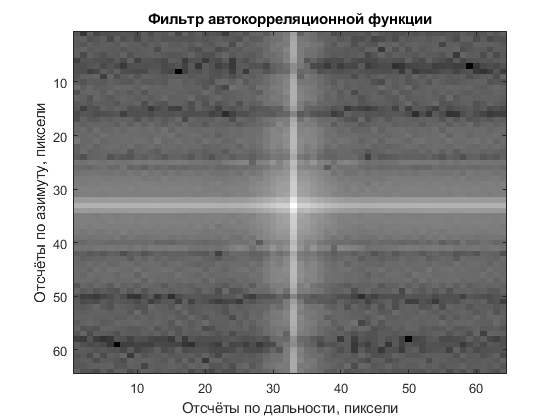
\includegraphics[width=0.8\textwidth]{acf.png}
    \caption{Автокорреляционная функция}
    \label{fig:acf}
\end{figure}


	При повороте точечной цели на некоторый угол, её АКФ также поворачивается, что позволяет учесть всевозможные напрвления "лучей". 	

\subsection{Алгоритм поиска псевдоточечных целей}

	На рисунке \ref{fig:alg_search_targets} представлена блок-схема алгоритма поиска псевдоточечных целей:

\begin{figure}[ht]
    \centering
    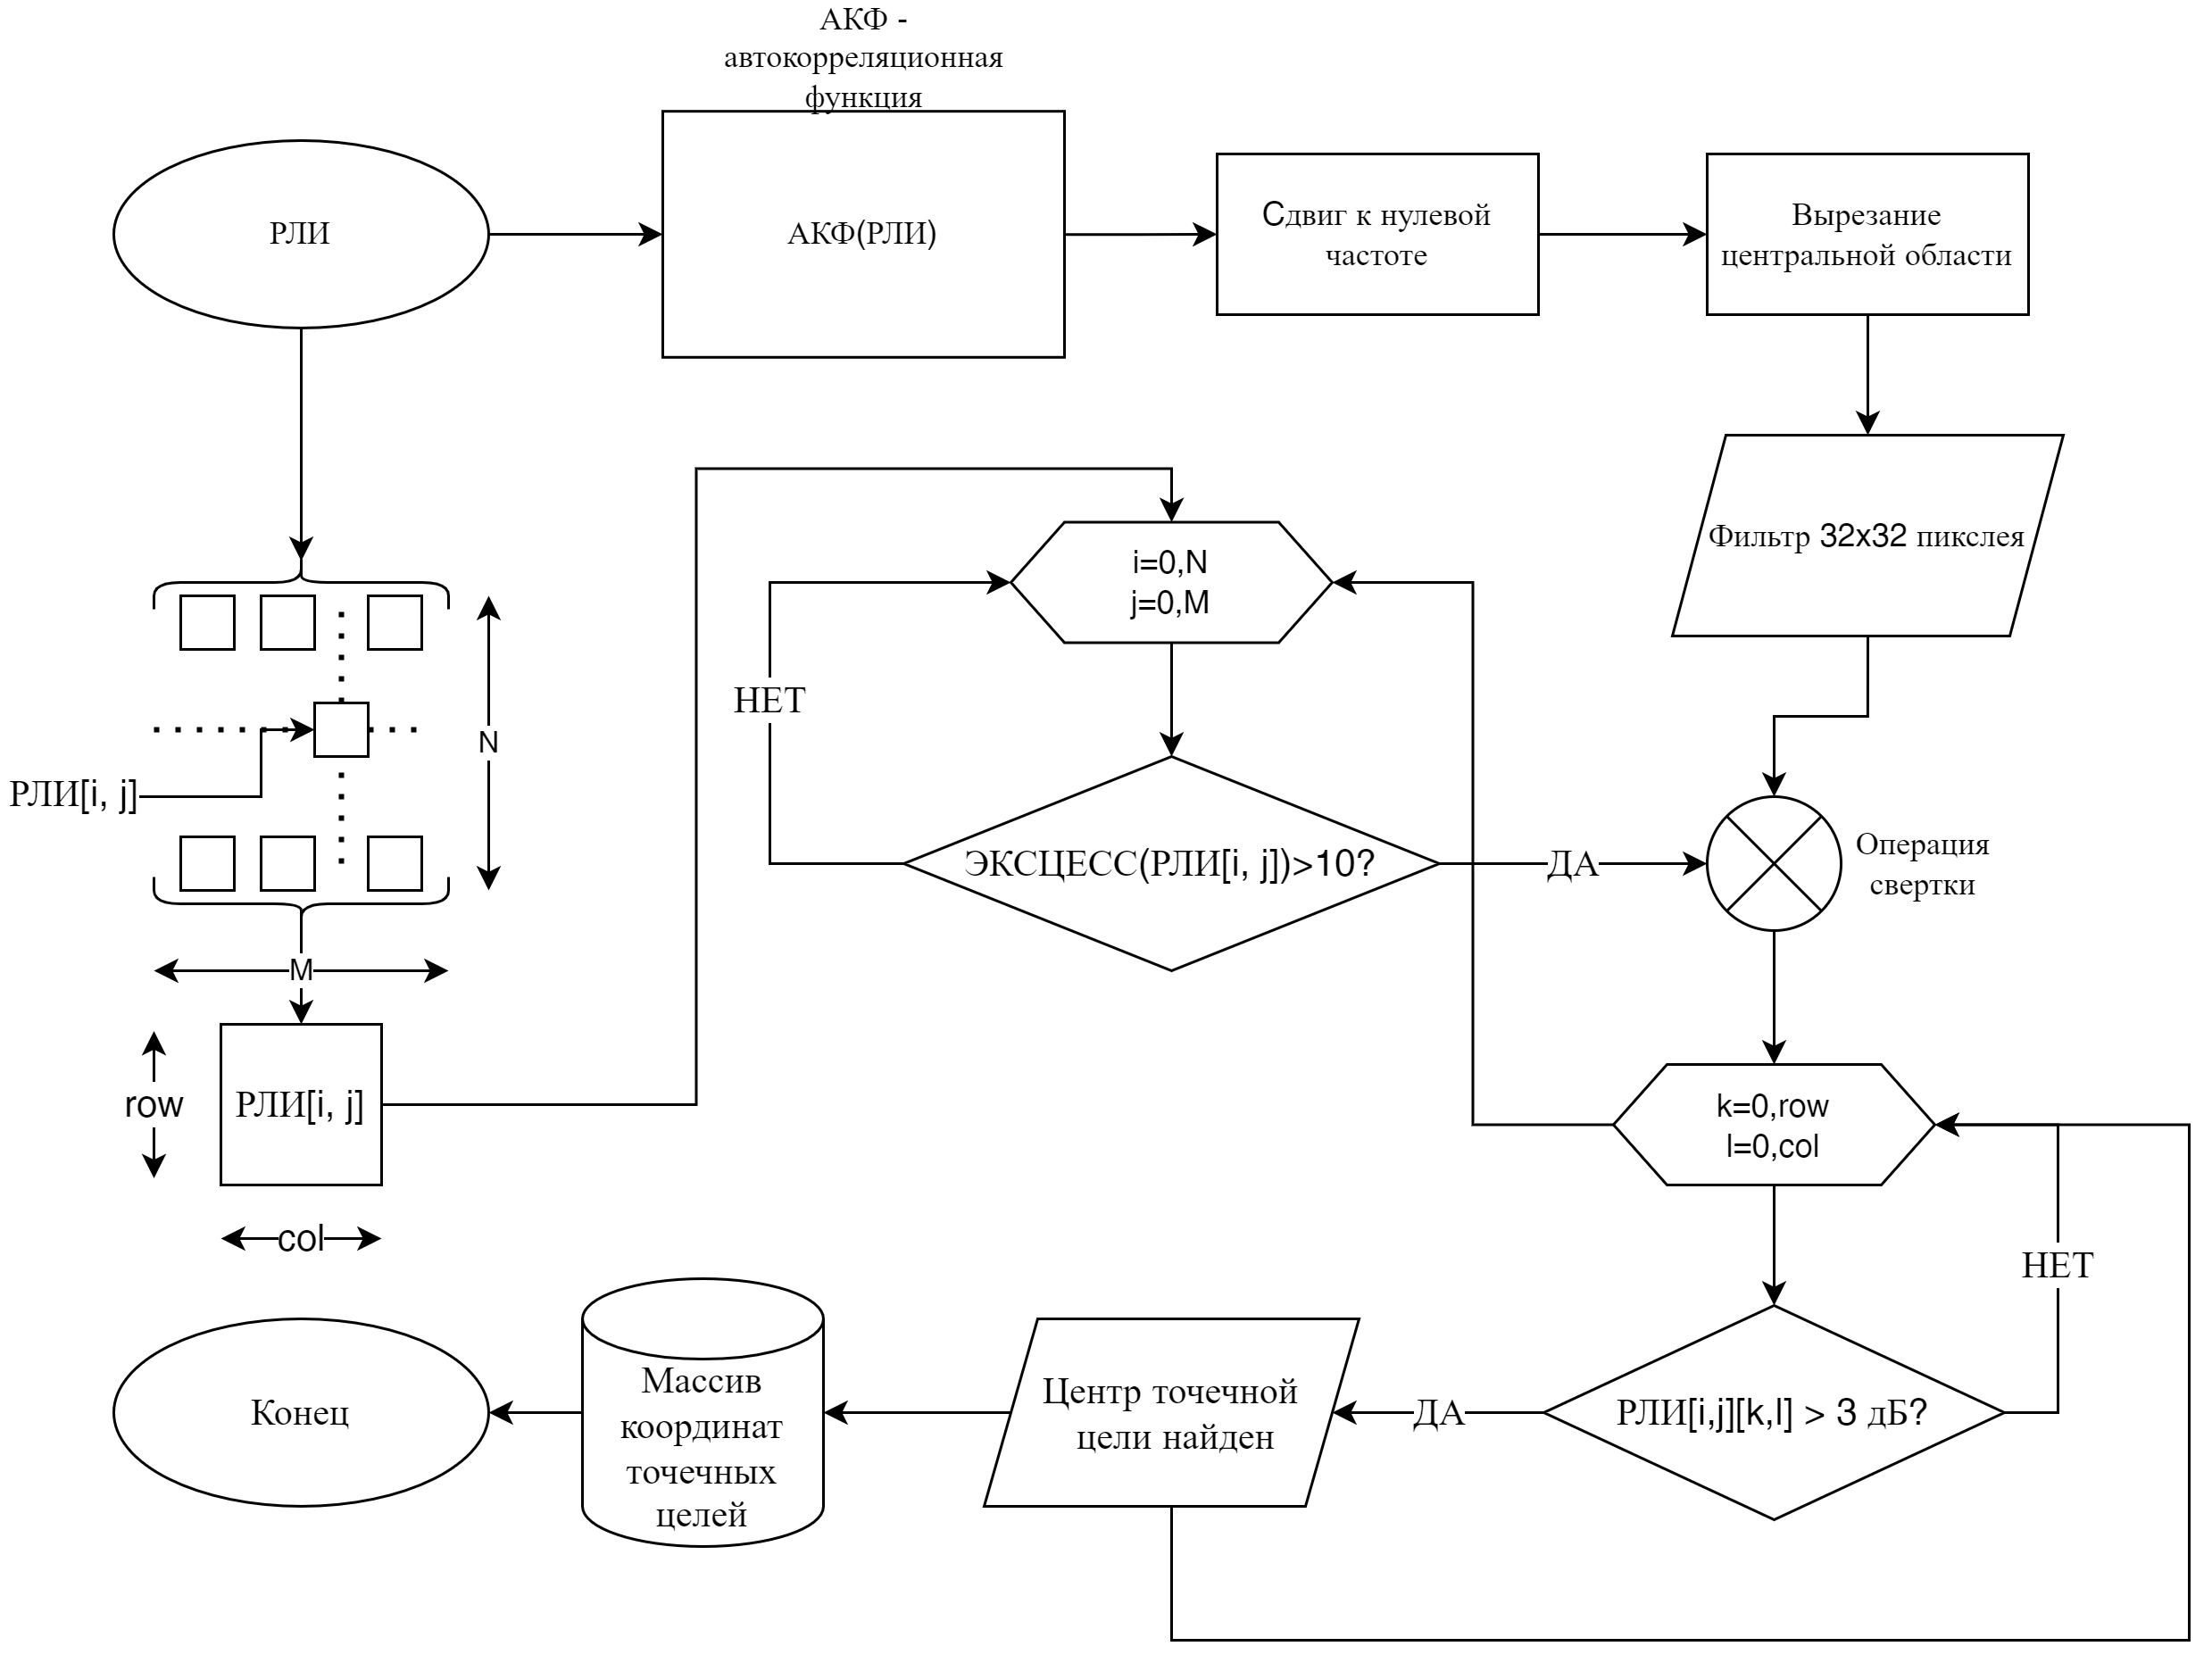
\includegraphics[width=1\textwidth]{alg_search_targets.png}
    \caption{Алгоритм поиска псевдоточечных целей}
    \label{fig:alg_search_targets}
\end{figure}

Она состоит из следующих шагов:

	1) Создание фильтра на основе автокорелляционной функции изображения
	
	2) Создание сетки на изображении с адаптивным шагом
	
	3) Вычисление статистического коэффициента ЭКСЦЕСС
	
	4) Отбор нужных клеток сетки по критерию ЭСЦЕСС > 10
	
	5) Вычисление свертки фильтра, полученного на 1 шаге, и отобранных областей
	
	6) Отбор значений пикселей по пороговому значению (данные пиксели являются центром точечных отражателей)

	Новизна представленного алгоритма заключается в использовании в качестве фильтра центр автокорреляционной функции изображения. Далее выполняется свёртка этого фильтра с наиболее информативными участками изображения. Это означает, что зашумленные или слабоотражающие участки нас не интересует, так как свертка с ними даст неопределенный результат. Поэтому для выделения наиболее информативных участков изображения используется статистический коэффициент ЭКСЦЕСС. Его особенность заключается в том, что он стремится к нулю при гауссовом распределении. Также была решена задача бинарной классификации, которая показала, что участки изображения с точечными целями c хорошим отношением сишнал/шум имеют значения ЭКСЦЕССА > 10. Далее после выполнения операции свертки пиксели отбираются по пороговому значению, это и будут центры точечных отражателей.		

\section{Алгоритм анализа отклика от псевдоточечных целей}

	Алгоритм анализа отклика от псевдоточечных целей ничем не отличается от анализа отклика от точечных целей. Согласно [Wong] наиболее важными характеристиками являются IRW (ширина главного лепестка по уровню -3дБ), PSLR (пиковый уровень боковых лепестков) и ISLR (интегральный уровень боковых лепестков). IRW явлется пространственным разрешением, а ISLR и PSLR отвечают за контраст.  
	

\begin{figure}[ht]
    \centering
    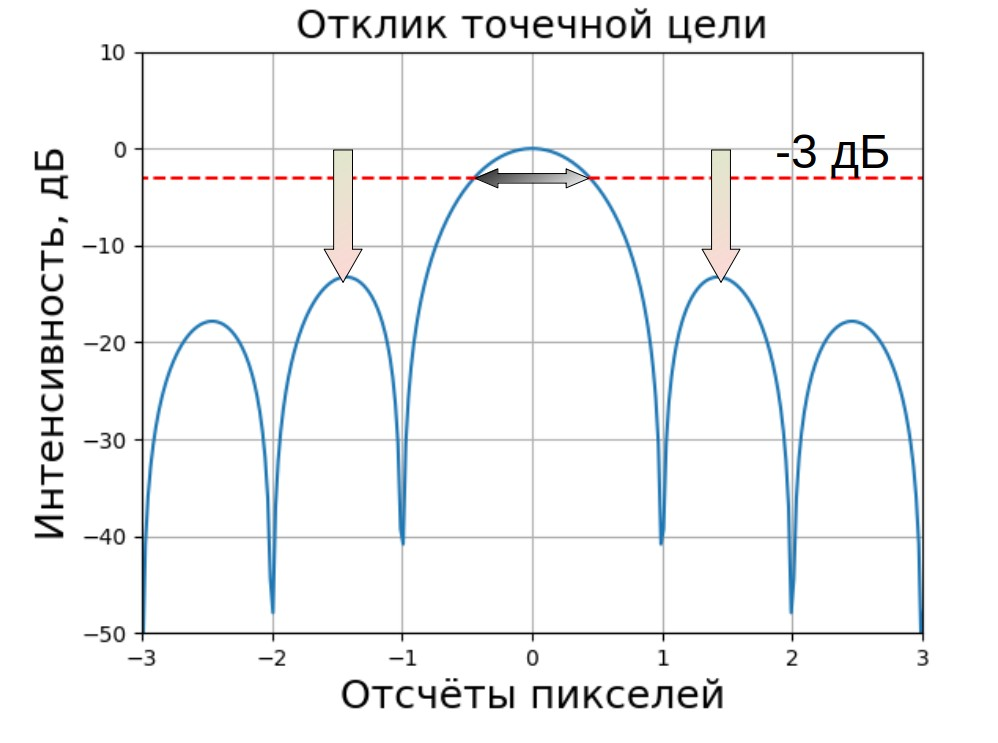
\includegraphics[width=0.8\textwidth]{metrics.png}
    \caption{Измерение характеристик по функции отклика}
    \label{fig:metrics}
\end{figure}
	
	На рисунке \ref{fig:alg_analys_targets} представлена блок-схема алгоритма анализа псевдоточечных целей. Она состоит из следующих шагов:
	
	1. Интерполяция исходного отклика методом добавления нулей в конец спектра.
	
	2. Определение направляющих осей по азимуту и по дальности.
	
	3. Вычисление проекции отклика на данные оси
	
	4. Расчёт требуемых характеристик по даннным проекциям
	
\begin{figure}[ht]
    \centering
    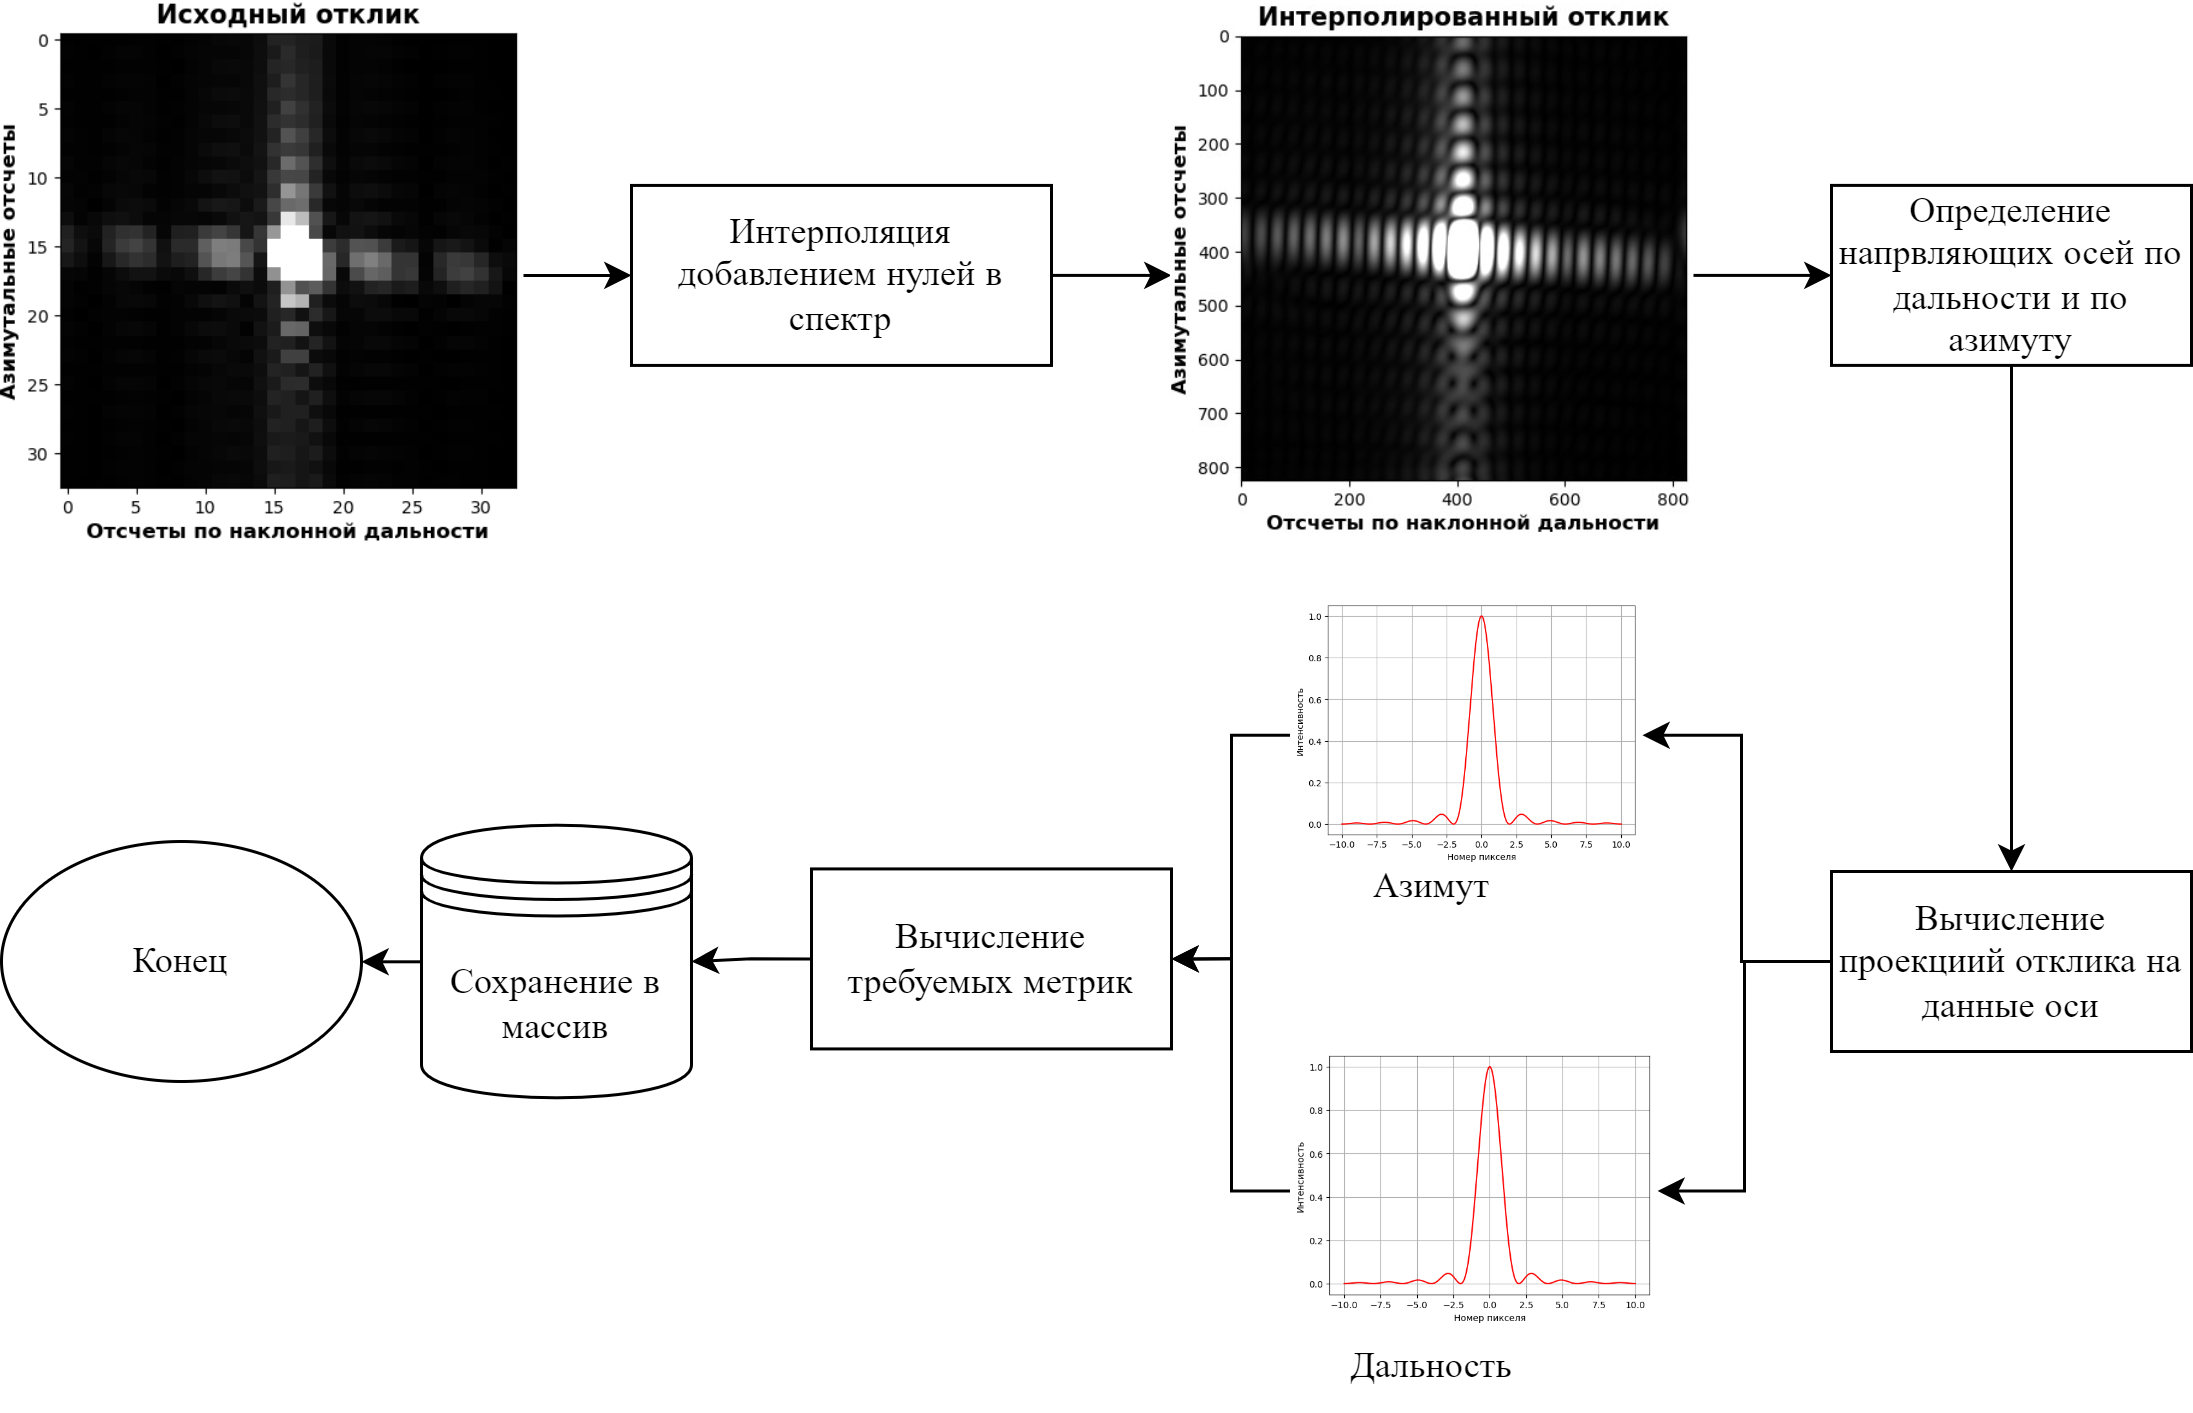
\includegraphics[width=1\textwidth]{alg_analys_targets.png}
    \caption{Алгоритм анализа псевдоточечных целей}
    \label{fig:alg_analys_targets}
\end{figure}

\section{Алгоритм автоматического поиска и анализа псевдоточечных целей}

	После объединения упомянутых выше алгоритмов и добавления статистического анализа распределений, итоговый алгоритм представлен на рисунке \ref{fig:alg}.

\begin{figure}[ht]
    \centering
    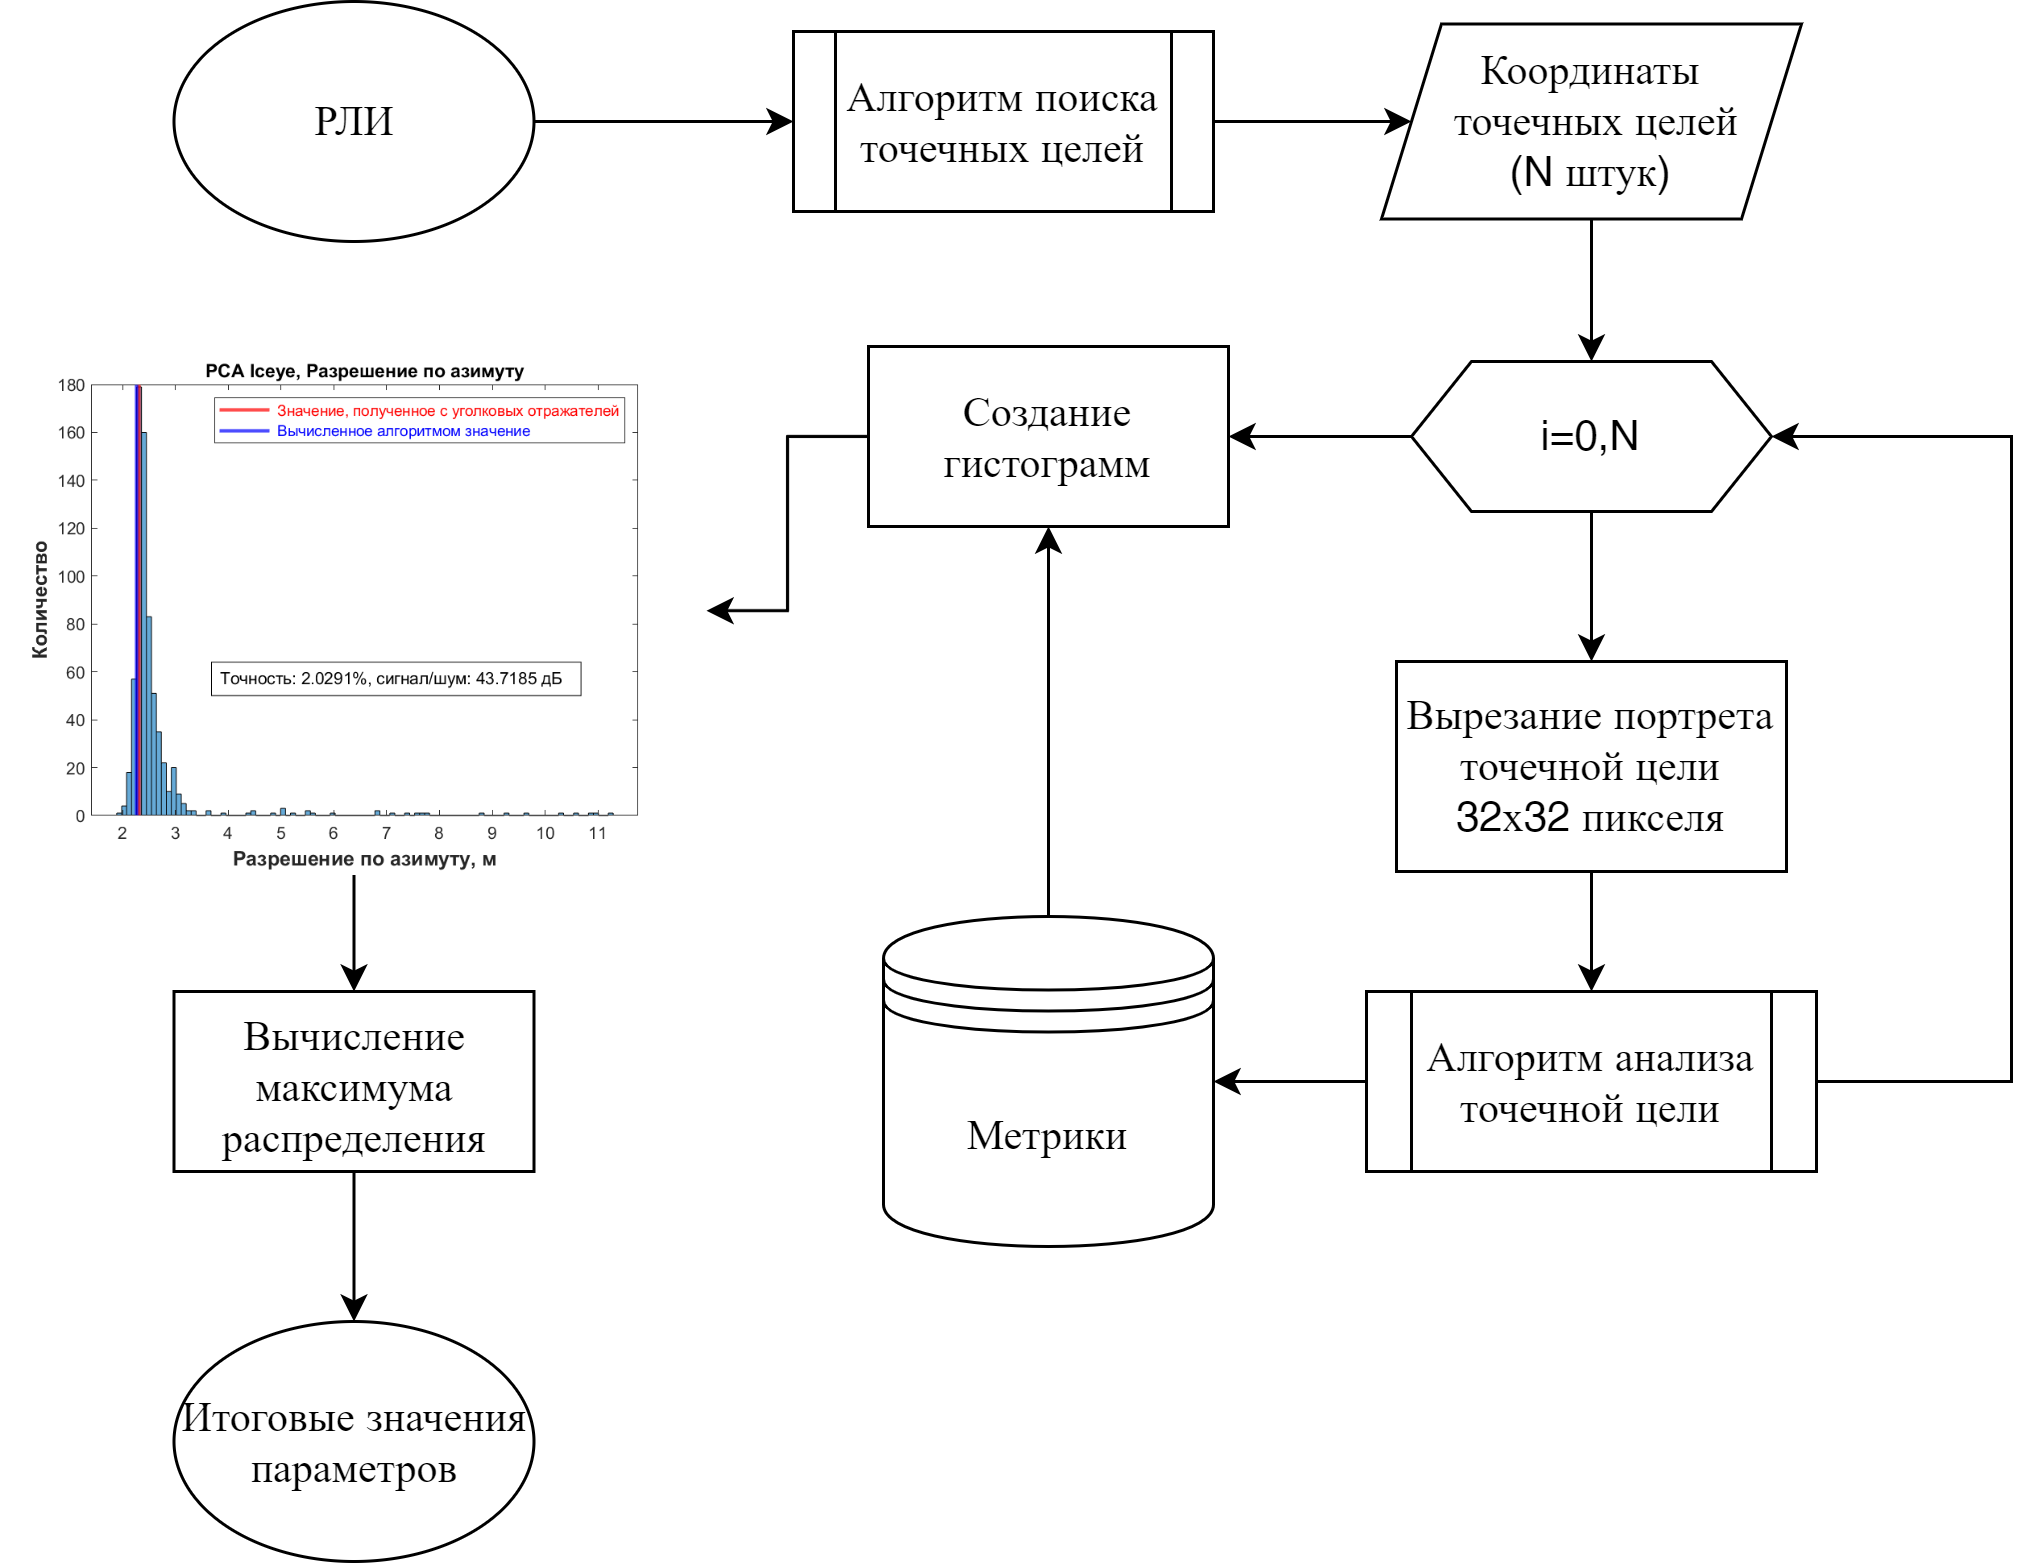
\includegraphics[width=1\textwidth]{alg.png}
    \caption{Алгоритм автоматического поиска и анализа псевдоточечных целей}
    \label{fig:alg}
\end{figure}

\newpage
